\section{Datasets}

\begin{table}[ht]
\centering
\caption{Overview of Datasets. Abbreviations: 'reg' = regression dataset; 'seg' = lane segmentation present; 'fid' = fiducial markers present; 'bal' = balanced classes (minority classes duplicated); 'Img+Q+L' = image, query, and label formatted for Vision Language Models. Datasets 16 and 17 were generated at inference time and not saved to disk. Total images: 1,917,822.}
\label{tab:datasets}
\begin{tabular}{l l r l}
\toprule
\textbf{ID} & \textbf{Dataset Name} & \textbf{Count} & \textbf{Description} \\
\midrule
1 & PMNIST & 1,200,000 & Perturbed MNIST \\
2 & MNISTified CIFAR-10 & 50,000 & Grayscale CIFAR-10 \\
3 & MNISTified English Handwritten Digits & 550 & Conformed to MNIST\\
4 & MNISTified English Handwritten Characters & 2,860 & Conformed to MNIST\\
5 & carla\_dataset\_640x480\_01 & 29,105 & reg, seg with fid \\
6 & carla\_dataset\_640x480\_02 & 29,108 & reg, seg \\
7 & carla\_dataset\_640x480\_03 & 29,105 & reg, fid only \\
8 & carla\_dataset\_640x480\_05 & 29,013 & seg 15 bins \\
9 & carla\_dataset\_640x480\_05\_bal & 152,996 & seg 15 bins bal \\
10 & carla\_dataset\_640x480\_06 & 27,114 & seg, 5 bins \\
11 & carla\_dataset\_640x480\_06\_bal & 79,206 & seg 5 bins \\
12 & carla\_dataset\_640x480\_07\_3\_bins & 26,954 & seg 3 bins \\
13 & carla\_dataset\_640x480\_07\_3\_bins\_bal & 67,391 & seg 3 bins bal \\
14 & carla\_dataset\_640x480\_07\_3\_bins\_qwen & 26,950 & seg 3 bin Img+Q+L \\
15 & carla\_dataset\_640x480\_07\_3\_bins\_qwen\_bal & 67,380 & seg 3 bin Img+Q+L \\
16 & CIFAR-10 (zero-shot) & 50,000 & 1440x1440 px (not saved) \\
17 & CIFAR-10 (zero-shot) & 50,000 & 720x720 px (not saved) \\
\midrule
& \textbf{Total} & \textbf{1,917,822} & \\
\bottomrule
\end{tabular}
\end{table}

Table \ref{tab:datasets} shows datasets created for this project. MNIST variants (IDs 1-4), including PMNIST and MNISTified datasets, were created for image classification using CNN and ViT models. CARLA simulator-generated datasets (IDs 5-15) were created for autonomous driving testing, including CNN/ViT regression models and CNN/ViT classification models with quantized steering angles (3, 5, and 15 bins). Figure \ref{fig:mnistified_cifar10} shows examples of the MNISTified CIFAR-10 dataset.

\begin{figure}[h]
\centering
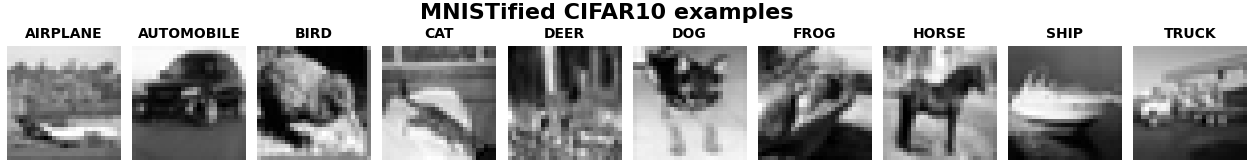
\includegraphics[width=0.99\textwidth]{Figures/Results/mnistified_cifar10.png}
\caption{Examples of the MNISTified CIFAR-10 dataset, where the RGB (three channel) images are converted to grayscale (single channel).}
\label{fig:mnistified_cifar10}
\end{figure}

For regression and classification models, the steering angle is embedded in the filename (e.g., \texttt{20250514\_154417\_678492\_steering\_0.0137.jpg}). The quantized steering angle datasets (3, 5, and 15 bins) use discrete values. For example, the 5-bin dataset uses values $-0.065$, $-0.015$, $0.000$, $0.015$, and $0.065$, corresponding to steering angles from $\pm$4.55 degrees, which is sufficient to navigate the figure-of-eight circuit in CARLA's Town04 map.

Datasets 14 and 15 extend datasets 12 and 13 by adding query prompts formatted for Vision Language Models. The system prompt instructs the model to act as a steering specialist and reply with only "Left", "Straight", or "Right" based on the provided image. The discrete steering angle labels ($-0.065$, $0.000$, $0.065$) were mapped to these natural language commands (Left, Straight, Right).

The VLM datasets (IDs 14 and 15) were used to fine-tune Qwen2-VL-2B-Instruct \cite{bai2023qwen} and deepseek-vl-1.3b-chat \cite{zeng2024deepseek} models. Datasets 16 and 17 were used for zero-shot evaluation with Llama-3.2-11B-Vision-Instruct \cite{meta2024llama3vision}.
